% This .tex source is an example which *does* use
% the .bib file (from which the .bbl file % is produced).
% REMEMBER HOWEVER: After having produced the .bbl file,
% and prior to final submission, you *NEED* to 'insert'
% your .bbl file into your source .tex file so as to provide
% ONE 'self-contained' source file.
%

\documentclass{sig-alternate}

\usepackage{algorithm}
\usepackage{algorithmic}

\begin{document}

\conferenceinfo{GECCO'14}{July 12-16,2014, Vancouver, BC, Canada.}
\CopyrightYear{2014}
\crdata{TBA}
\clubpenalty=10000
\widowpenalty=10000

\title{Is it possible to generate good Earthquake Risk Models using Genetic Algorithms?}

\numberofauthors{4} 

\author{
\alignauthor Blind Author 1\\
       \affaddr{University 1}\\
       \affaddr{Address 1}\\
       \affaddr{Address 2}\\
       \email{e-mail@address.com}
\alignauthor Blind Author 2\\
       \affaddr{University 1}\\
       \affaddr{Address 1}\\
       \affaddr{Address 2}\\
       \email{e-mail@address.com}
\and
\alignauthor Blind Author 3\\
       \affaddr{University 1}\\
       \affaddr{Address 1}\\
       \affaddr{Address 2}\\
       \email{e-mail@address.com}
\alignauthor Blind Author 4\\
       \affaddr{University 1}\\
       \affaddr{Address 1}\\
       \affaddr{Address 2}\\
       \email{e-mail@address.com}
}

\date{29 January 2014}


\maketitle
\begin{abstract}
Understanding the mechanisms and patterns of earthquake occurrence is of
crucial importance for assessing and mitigating the seismic risk. In this
work we analyze the viability of using Evolutionary Computation (EC) as a
means of generating models for the occurrence of earthquakes. Our proposal
is made in the context of the "Collaboratory for the Study of Earthquake
Predictability" (CSEP), an international effort to standardize the study
and testing of earthquake forecasting models.

We use a standard Genetic Algorithm (GA) with real valued genome, where
each allele corresponds to a bin in the forecast model. The design of an
appropriate fitness function is the main challenge for this task, and we
test three different proposals, all based on the log-likelihood of the
candidate model against the training data set.

The resulting forecasting models are compared with statistical models
traditionally employed by the CSEP community, using data from the
Japan Meteorological Agency (JMA) earthquake catalog. Our results
indicate promise for the use of GA as basis for constructing
statistical earthquake forecast models. Based on these results, we
identify research directions that we consider deserve more attention
from the EC community.
\end{abstract}

% A category with the (minimum) three required fields
\category{I.2.8}{Artificial Intelligence}{Problem Solving, Control
  Methods and Search Heuristic Methods}
%A category including the fourth, optional field follows...
\category{J.2}{Computer Application}{Physical Sciences and
  Engineering}[Earth and Atmospheric Sciences]

\terms{Real World Applications}

\keywords{Earthquakes, Risk Models, Genetic Algorithms, Forecasting}

\section{Introduction}

Earthquakes pose a huge risk for human society, in their potential for
large scale loss of life and destruction of infra-structure. In the
last decade, large earthquakes such as Sumatra (2004), Kashmir (2005),
Sichuan (2008) and Tohoku (2011) caused terrible amounts of casualties.

Therefore, it is crucially important to understand the patterns and
mechanisms behind the occurrence of earthquakes. These may allow us to
create better seismic risk forecast models, with general information
about about when and how often large earthquakes are expected to
happen. Such information can be put to good use for mitigating damage
through urban planning, civil engineering codes, emergency
preparedness, et cetera.

%TODO:
% - Outline of earthquake model research
% - Prediction models
% -- RELM and CESP

% - GA contributions (a few in other 


** However, the specifics of earthquake generation mechanisms are not
yet completely understood. In this sense, the development of accurate
models for the risk assessment of earthquake activity is a very active
area of study.

** In the study of Earthquake predictability, we highlight the RELM
(Relative Earthquake Log-likelihood Model) and the CSEP

**** Evolutionary algorithms have shown themselves to be very
effective in hard problems, such as (...). However, the use of EC
techniques in seismology studies, and in particular in the development
of earthquake risk models, is extremely scarse.

** We believe that a real contribution can be make by the use of
evolutionary techniques in this field. Therefore in this paper we ****
make a tutorial on earthquakes,

*** We illustrate these ideas by designing a simple genetic algorithm
that creates an earthquake prediction model as defined by the CSEP. We
compare this algorithm with a ``skilless'' model (random model), and
the RI model. Using Data from the JMA catalog between 2000 and 2012

** Our Results

-- Our main goal is to understand X

** Outline of the paper
In section 2, we describe the Earthquake predictability problem.


%%%%%%%%%%%%%%%%%%%%%%%%%%%%%%%%%%%%%%%%%%%%%%%%%%%%%%%%%%%%%%%%%%%
\section{The Earthquake Prediction Problem}

(WRITE) What is the Earthquake Prediction Problem

%% What is the CSEP
In this context, the Collaboratory Study for Earthquake Predictability
(CSEP) is a global project to support rigorous research into the
forecast models of earthquake rupture processes.  

%% What does it do

%% Why it is important for us

In order to objectively compare forecasts 

\subsection{Earthquake Forecast Model}\label{CSEP_definition} 
%% TO REVIEW

\begin{figure}
  \begin{center}
    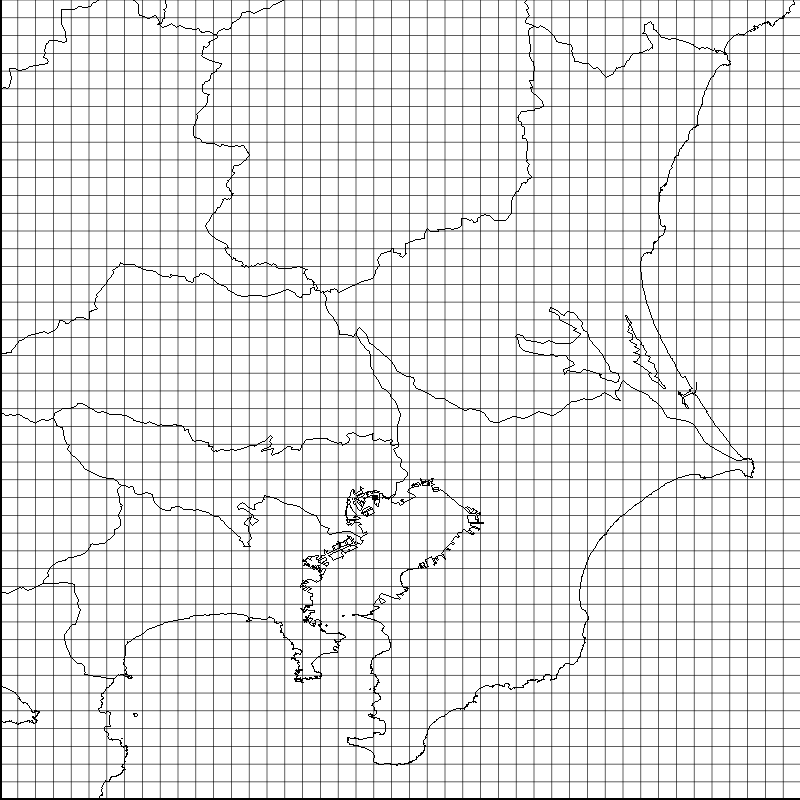
\includegraphics[width=0.45\textwidth]{img/kantomap.png}
  \end{center}
  \caption{Target area for the Kanto region and its bins}
  \label{fig:kantomap}
\end{figure}

The forecast target is defined as a geographical region, a starting
date and an ending date. A forecast model will estimate the number
(and sometimes the magnitude) of earthquakes happening within this
target time/space.

A forecast is composed of \emph{bins}. Each bins represents a
geographical interval, measured in latitude and longitude, and
sometimes a magnitude interval. 

For example, in this paper we define the ``kanto'' region as as the
area covered by latitude N34.8 to N36.3, and longitude E138.8 to
E140.3. This area is divided into 2025 (45x45) bins of approximately
$5km^2$ (Figure~\ref{fig:kantomap}).

For each bin in the forecast we associate a (positive, integer) number
of expected earthquakes for that bin. A good forecast is that which
the number of estimated earthquakes in each bin corresponds to the
actual number of earthquakes that occurs in the target time period.

\subsection{The CSEP Tests} 
%% TO REVIEW, 2nd paragraph can be reduced if needed.

The CSEP framework uses six different tests to compare earthquake
forecasts. These are divided into two groups: log-likelihood based
tests, and alarm based tests.

Log likelihood tests are based on a direct analysis of the similarity
between the forecast and the actual earthquake
catalog~\cite{Schorlemmer2007}. A Poissonian probability distribution
function is used to measure the likelihood between the forecast and
the data. Three statistical tests are defined using this metric: the
\emph{L-test}, which compares a forecast with the data, the
\emph{N-test}, which compares the total number of earthquakes forecast
with the total number of observed earthquakes, and the \emph{R-test},
which compares multiple forecasts at the same time. These tests
require that all the forecasts being compared have the same number and
size of bins.

Alarm based tests, on the other hand, are based on a treshold
analysis~\cite{Zechar2010}. All bins with forecast values above the
treshold are added to an ``alarm set''. The tests generate two values:
a miss rate $v$, the proportion of earthquakes in the data that
occurred in bins outside the alarm set; and the coverage rate $\tau$,
the proportion of the total bins in the model covered by the alarm
set. Three alarm based tests are defined: the \emph{Molcham Diagram}
draws a path of $v$ and $\tau$ based on varying values of the
treshold, the \emph{Area Skill Score (ASS)} summarizes a Molcham
Diagram into a single number. A Receiver Operating Characteristic
(ROC) can also be drawn using method of analysis. These testes do not
take into account the total number of earthquakes, either from the
forecast or the data.

\subsection{The Relative Intensity Algorithm}
%% TO REVIEW

The Relative Intensity (RI) algorithm is a commonly used benchmark for
earthquake prediction models~\cite{Nanjo2011}. In this paper, we use
it as goalpost to assess the suitability of evolutionary computation
for this problem.

The working assumption behind the RI is that larger earthquakes are
more likely to occur at locations of high seismicity in the
past. Accordingly, the RI algorithm will estimate the number of
earthquakes in a bin based on the number of earthquakes observed in
the past for that bin, plus an attenuation factor that takes into
account the seismicity of neighboring bins.

For more details on the implementation of the RI, please see the paper
by Nanjo~\cite{Nanjo2011}. In the experiments in this paper, we use
the following parameters: $b = 0.8$ and $s = 5$.

\section{Evolutionary Computation for Earthquake Risk Analysis}
%% TO REVIEW, needs to merge with Yuri's data

In the field of seismology and earthquake risk analysis, the few cases
of Evolutionary Algorithm approaches have usually taken one of two
forms. EC is often used to estimate parameter values for seismological
models.  These models can be used to describe and understand
earthquakes.

For example, Ramos~\cite{Ramos2011} uses Genetic Algorithms to decide
the location of sensing stations in a seismically active area in
Mexico. Nicknam et. al~\cite{Nicknam2010} and Kennett and
Sambridge~\cite{Kennett1992} used evolutionary computation to
determine the Fault Model parameters (such as epicenter location,
strike, dip, etc) of a given earthquake. Evolutionary Computation has
also been used to estimate the peak ground accelleration of
seismically active areas~\cite{Kermani2009, Cabalar2009}.

EC has also been used very few times as a method to generate seismic
forecast model. One such approach is described by Zhang and
Wang~\cite{Zhang2012}, where they fine tune a Neural Network with a
GA, and then use this system to produce a forecast. Unfortunately that
work did not provide enough information to reproduce the proposed
GA+ANN system or their results.

\section{A Forecast Model Using Genetic Algorithms} 
%% TO REVIEW

To investigate the ability of Evolutionary Computation to generate
earthquake forecast models, we design and test a simple Genetic
Algorithm. Let us call this system the \emph{GAModel}.

An individual in GAModel will encode a forecast model as defined in
the CSEP framework~(\ref{CSEP_definition}). The population will be
trained on earthquake occurrence data for a fixed training period. The
best generated individual will be compared with a model generated by
the RI algorithm, and a skilless (random) model. This comparison is
based on earthquake occurrence data for a test period immediately
posterior to the training period.

By encoding the entire forecast model as one individual, we identified
two main concerns while designing GAModel: First, as the forecast
model contains a large number of bins, the genome of an individual
will be respectively large. Evolutionary operators and parameters must
be chosen carefully to guarantee convergence in a reasonable time, and
avoid local optima.

Secondly, the design of the fitness function deserves a lot of
attention, to avoid the risk of the system overfitting to the training
data.

\subsection{Genome Representation}
%% TO REVIEW
% IF space: add that mu can be adjusted if the intervals of test and
% train are different.
% IF space: might want to add a review of the bin definition

In GAModel, each individual represents an entire forecast model. The
genome is a real valued array $X$, where each element corresponds to
one bin in the desired model (the number of bins $n$ is defined by the
problem). Each element $x_i \in X$ can take a value from $[0,1)$. In
  the initial population, these values are sampled from a uniform
  distribution.

In the CSEP framework, a model is defined as a set of integer valued
expectations, corresponding to the number of predicted earthquakes for
each bin. To convert from the real valued chromossome to a integer
forecast, we use a modification of the Poisson deviates extraction
algorithm from~\cite{NumericalRecipes}~(Chapter 7.3.12).

\begin{algorithm}
  \caption{Obtain a poisson deviate from a $[0,1)$ value}
  \label{InversePoisson}
  \begin{algorithmic}
    \STATE Parameters $0 \leq x < 1, \mu \geq 0$
    \STATE $L \gets \exp{(-\mu)}, k \gets 0, prob \gets 1$
    \REPEAT 
    \STATE $\text{increment }k$
    \STATE $prob \gets prob*x$
    \UNTIL{$prob > L$}
    \RETURN $k$
  \end{algorithmic}
\end{algorithm}

In Algorithm~\ref{InversePoisson}, $x$ is the value taken from the
chromossome, and $\mu$ is the average number of earthquakes observed
across the entire training data. Note that in the original algorithm,
$k-1$ is returned. Because the log likelihood calculation used for
model comparison discards forecasts that estimate $0$ events in bins
where earthquakes are observed, we modify the original algorithm here
to make sure all bins estimate at least one event.

%% TODO: If We have space -- Explain that \mu is resized if the time
%% intervals are different between the training and the testing data
%% sets.

\subsection{Fitness Function}

The main challenge when applying an Evolutionary Computation method to
any new application domain is usually the definition of an appropriate
fitness function. Accordingly, the largest part of our effort in this
work was to define a good fitness function for GAModel.

\subsubsection{Simple Log Likelihood Fitness Function} %% DONE

Our first candidate was the log-likelihood between the forecast
generated by an individual and the observed earthquakes in the
training data, as described by Schorlemmer
et. al.~\cite{Schorlemmer2007}. In simple terms, the log likelihood is
a measure of how close a forecast is to a given data set.

Let $\Lambda = \{\lambda_1, \lambda_2, \dots, \lambda_n | \lambda_i
\in \mathbb{N}\}$ be a forecast with $n$ bins. In this definition,
$\lambda_i$ is the number of earthquakes that is forecast to happen in
bin $i$. To derive $\Lambda_X$ from an individual $X = \{x_1, x_2,
\dots, x_n | 0 \leq x_i < 1\}$, we calculate each $\lambda_i$ from
$x_i$ using Algorithm \ref{InversePoisson}.

Let $\Omega = \{\omega_1, \omega_2, \dots, \omega_n | \omega_i \in
\mathbb{N}\}$ be the observed earthquakes in the training data. The
log likelihood between an individual's forecast $\Lambda_X$ and the
observed data $\Omega$ can be calculated as:
\begin{equation}
  L(\Lambda_X|\Omega) = \sum_{i=0}^n {-\lambda_i +
    \omega_i*\ln(\lambda_i)-ln(\omega_i!)}
\end{equation}
There are two special cases that arise when any $\lambda_i = 0$. If
$\lambda_i = 0$ and $\omega_i = 0$, then the value of the sum for that
element is $1$. If $\omega_i > 0$, then $L(\Lambda_X|\Omega) =
-\infty$ and the forecast must be discarded. For more details on
this, see~\cite{Schorlemmer2007}.

In the Simple Log Likelihood fitness function, the value of
$L(\Lambda_X|\Omega)$ is taken as the fitness value of the individual.

Early testing with the Simple Log Likelihood function showed that
GAModel had a very strong tendency to overfit to the training
data. This is natural, since there are differences between the
seismocity of a larger period and a shorter one. 

To avoid this overfitting, we have developed two alternative fitness
functions.

\subsubsection{Simulated Log Likelihood Fitness Function} %% DONE

In the Simulated Log Likelihood fitness function, we generate $k$
``simulations'' from the observed data $\Omega$, and compare an
individual's forecast with all the simulated data.

Let $\hat\Omega =
\{\hat\omega_1,\hat\omega_2,\dots,\hat\omega_3
|\hat\omega_i\in\mathbb{N}\}$ be a simulated data set generated from
$\Omega$. Each $\hat\omega_i$ is taken randomly from a Poissonian
distribution with mean $\omega_i$.

To calculate the Simulate Log Likelihood fitness, we calculate the Log
Likelihood of the forecast $\Lambda_X$ generated by an individual $X$
against each of the $k$ simulated data sets
($L(\Lambda_X|\hat\Omega_1), \dots, L(\Lambda_X|\hat\Omega_k)$). We
use the lowest of the $k$ log likelihood values as the fitness of $X$.

The idea behind this fitness function is that by training against a
number of similar, but slightly different training data sets at the
same time, we might be able to avoid overfitting the forecast to the
observed training data set.

\subsubsection{Time-slice Log Likelihood Fitness Function} %% DONE

In the time-slice log likelihood fitness function we break up the
training data set into smaller \emph{slices}. These slices are based
on the chronology of the earthquakes contained in the training
catalog. The duration of each slice is the same as the duration of the
test catalog.

Let's consider an example where the target period for the forecast is
one year, from 1/1/2014 to 1/1/2015, and the training data is taken
from the 10 year period of 1/1/2004 to 1/1/2014. The time-slice log
likelihood fitness function will divide the training data into ten
1-year periods, from 2004 to 2005, 2005 to 2006, and so on. 

When an individual $X$ is evaluated, we calculate the log likelihood
of its forecast $\Lambda_X$ against each of the time slices
($\Omega_{2004}, \Omega_{2005}, \dots, \Omega_{2013}$). The lowest
value is used as the fitness of $X$.

The idea behind this fitness function is that the catalog data
available for training will normally span a period of time much longer
than the desired forecast. By breaking the training data into smaller
periods, we are trying to make the evolutionary algorithm learn any
time-repeating pattern that might exist in the data.

\subsection{Evolutionary Operators and Parameters} %% DONE

GAModel uses a regular generational genetic algorithm. For selection,
we use Elitism and Tournament selection. 

For the crossover operator we use \emph{aNDX}, recently proposed by
Someya~\cite{Someya2013}. If the value of a chromossome after the
crossover falls outside the $(0,1]$ boundary, it is truncated to these
  limits. For the mutation operator, we sample entirely new values
  from $(0,1]$ for each mutated chromossome.

\begin{table}[!h]
  \begin{center}
  \begin{tabular}{|l|r|}
    \hline
    Population Size & 500\\
    Generation Number & 100\\
    Elite Size & 1\\
    Tournament Size & 50\\
    Crossover Chance & 0.9\\
    aNDX parents & 4\\
    aNDX zeta & 0.5\\
    aNDX sigma & 1\\
    Mutation Chance (individual) & 0.8\\
    Mutation Chance (chromossome) & (genome size)$^{-1}$\\
    \hline    
  \end{tabular}
  \end{center}
  \caption{Parameters for GAModel}
  \label{GAParameters}
\end{table}

The parameters used for the evolutionary computation are described in
Table~\ref{GAParameters}. At this stage, we are not yet particularly
worried with convergence speed of the system. Because of this, not a
lot of effort was spent fine tuning these paremeter's values. Instead,
these values were choosen by trial and error on a data region not used
in the experiments of section~\ref{data}, until an acceptable
convergence time was found.

%% TODO: Overfitting comparison between the three fitness functions.

\section{Experiments}
%% TODO: Introduction to Experiments section
%% TODO: Goals of our experiments
%% Outline of the experiments

\subsection{Experimental Data}\label{data}

The data used in these experiments comes from the Japan Meteorological
Agency's (JMA) catalog. The catalog lists earthquakes recorded by the
sensing station network in Japan, along with the time, magnitude,
latitude, longitude and depth of the hypocenter.

The part of the catalog used in this work spans a period from 2000 to
2013, and has over 220.000 earthquakes recorded in the Japanese
archipelago. In order to better understand the predictive power of
GAModel, we divide the catalog into 5 areas, which are used in the
experiments below. The relative position and size of these areas can
be seen in Figure~\ref{areamap}.

\begin{enumerate}
  \item {\bf All Japan:}
  \item {\bf Sendai:}
  \item {\bf Kantou:}
  \item {\bf Kansai:}
  \item {\bf Touhoku:}
\end{enumerate}

%% TODO: Geographical Description of the Data (depth, number of bins, reasoning)
%% TODO: Figures of the locations we chose for the experiments

\subsection{Experimental Design} %% DONE

To test the ability of a Genetic Algorithm to generate an effective
earthquake risk model, we perform a forecast experiment. In this
experiment we compare three forecasts: a randomly generated forecast,
one generated by the RI algorithm, and a group of forecasts generated
by the proposed method.

We define a ``scenario'' as a region and a forecast period. In this
experiment, we will test 5 regions (all japan, pacific, kanto, tohoku,
kansai), and 7 one-year periods (from 2005 to 2012), for a total of 40
scenarios.

Each scenario has a corresponding training window, which consists of
the 5 years prior to the scenario's forecast time. This training
period is used by the RI algorithm and by the proposed method to
generate their respectives forecasts. For the sake of statistical
testing, we generate 20 forecasts using the GAModel. Unless noted
otherwise, all results reported are an average of these runs.

%% TODO: Remove ASS if we end up not using it.
We compare the forecasts in three different ways: Using the
log-likelihood between the forecast and the testing data, Using the
ASS value, and visually by comparing the forecast maps of some
significative scenarios.

\subsection{Results and Comparison of forecast models}

%% TODO: Table with all the log likelihood results
%% Indicate whether the difference between RI and GA is statistically significant

%% TODO: Table with the ASS results
%% Indicate whether the difference between RI and GA is statistically significant

%% TODO: Choose some scenarios (maybe 3?) to visually compare

%% TODO: If there is not enough space, indicate that extra results
%% will be left as additional material

%% TODO: Justify the use of Molcham Diagrams and ASS

\section{Conclusion}

%% TODO: Conclusions and Future Work

-- We choose the parameters hapzardly - a more careful parameter
selection might improve the result (or at least the running time)


-- There is a large number of problems related to the development of
forecast models: Parameter optimization, model construction,
earthquake clustering, etc.

-- On the evolutionary side, we think GA or ANNs might be a good idea.

-- We encourage people to work on this with us.

\subsection{Future Work}




\section*{Acknowledgements}

TODO: Check with Bogdan if we need to provide Acknowledgements for the
JMA data.

% initial runs of your .tex file to
% produce the bibliography for the citations in your paper.
\bibliographystyle{abbrv}
\bibliography{earthquake}

%\balancecolumns
\end{document}
